\documentclass[a4paper,12pt]{article}
\addtolength{\oddsidemargin}{-1.cm}
\addtolength{\textwidth}{2cm}
\addtolength{\topmargin}{-3cm}
\addtolength{\textheight}{3.5cm}
\makeindex


\usepackage[pdftex]{graphicx}
\usepackage{makeidx}
\usepackage{hyperref}
\hypersetup{
    colorlinks=true,
    linkcolor=blue,
    filecolor=magenta,      
    urlcolor=cyan,
}


% define the title
\author{Team Delta}
\title{ Assignment 1}
\begin{document}
\setlength{\parskip}{6pt}

% generates the title
	\begin{titlepage}
		\begin{center}
			
\includegraphics[width=1\textwidth]{./up-logo.jpg}\\[1.5cm] 
			\textsc{\LARGE Department of Computer Science} \\ [.5cm]
			\textsc{\Large COS 301 - Mini Project} \\ [.5cm]
			\textsc{\Large Assignment 1} \\ [.5cm]
			\line(1,0){450}\\[.5cm]
			\huge{\bfseries Software Requirements Specification and Technology Neutral Process Design}\\
			\line(1,0){450}\\[.5cm]
			\textsc{\LARGE Team Delta}\\ [0.5cm]
			
			
			\textsc{\small Mpho Sharon Baloyi (14133670)}\\
			\textsc{\small Dirk de Klerk (28159102)}\\
			\textsc{\small Killian Kieck (12252213)}\\
			\textsc{\small Daniel Malangu (13315120)}\\
			\textsc{\small Dzilafho Mulugisi (13071603)}\\
			\textsc{\small Duncan Smallwood (13027205)}\\
			\textsc{\small Dian Veldsman (12081095)}\\
			
			
			
			
			
		\end{center}
	\end{titlepage}
	
\tableofcontents
\thispagestyle{empty}
\footnotesize
\normalsize




\newpage
\section{Introduction}

This document aims to set out the functional and non-functional requirements of a system as specified by the Department of Computer Science. The system is required to allow the department to collaborate, share, and maintain research articles in an effective and efficient manner. The document will also serve the purpose of communicating the requirements and specifications as needed by the client.

\newpage
\section{Vision}

The client for this project, Department of Computer Science, has called for the design of an application that will allow the department to keep track of all research publications written and published within the department. The main idea behind the project is to alleviate the stress and time required for collaborating on, maintaining, and completing research articles. We have therefore invisioned the following goals:

	\begin{itemize}
		\item[$\bullet$] Simplify the effort required in maintaining publications as well as pending works.
		\item[$\bullet$] Ability to add/remove/specify main author and co-authors.
		\item[$\bullet$] Keep track of impact scores of different publications
		\item[$\bullet$] Allow authors and staff members to collaborate on articles.
		\item[$\bullet$] The ability to add/remove/edit meta-data of said articles.
		\item[$\bullet$] Allow different levels of privilege on user accounts.
		\item[$\bullet$] Afford privileged users (HODs) the ability to access addtional information on authors, publications and/or a summary page.  
		\item[$\bullet$] The need to integrate the software in android or web based applications.
		\item[$\bullet$] Afford only head authors the ability to remove co-authors as well as transfer authorship.
	\end{itemize}
	
\newpage
\section{Background}

We find ourselves within the Information Age which means we are bombarded with more information than we can handle. This implies the rise of new challenges. How does one deal with this information overload in a timely and effective manner? Technology is the primary cause of the problem but at the same time provides us with multiples solutions in the form of networking. 

The very nature of research means that a team or individual will constantly have to revise and apply changes to their work as new information becomes available. Some research efforts are simply to large handle on an individual level as is the case with interdiciplinary and cohort studies. Thus effective team work is required. When team members find themselves in remote locations, this can lead to a serious problem. How does one succesfully collaborate effectively and efficiently?

The above problem is what is currently hindering research efforts within the Department of Computer Science and the world! It is for this reason that the client is interested in developing a research repository that will allow them to share, maintain, and collaborate on various research papers in an effective and timely manner. A system, that is easy to use, is thus suggested to enable remote collaboration on research materials allowing the user to save considerably on time and effort. Such a system would certainly improve the throughput of research efforts, thus allowing authors to focus on quality research rather than deadlines.  

\newpage
\section{Architecture Requirements}
\subsection{Access Channel Requirements}
\begin{flushleft}

This section specifies and describes different access channels through which the services of the target system will be accessed by humans. The different functions of the system will be highlighted and how different access channels will provide access to these functions. The system must be able to provide the platforms with an interface through which they can access the functions this will be done through the use of a Application Programming  Interface (API).

To access the services of the systems users have to be connected to a network preferably the internet instead of a LAN, this is to enable users to access the services of the system from anywhere around the world. The type of devices that will enable access to the system's services are devices capable of connecting to the internet.

To provide access to the services of the system, the client requested that the following platfroms
be used:

\begin{itemize}
\item[$\bullet$]A Web Interface
\item[$\bullet$]An Android Application
\\
\end{itemize}
 
The above mentioned platforms will have ways of providing the functionality of the system through their methods that are defined in their API's. The access channels will have to provide the users with the ability to view certain data structures , search through the data structures, create new entities (users and publication meta-data ), delete existing entities, update attributes of existing entities , to open, view, edit or import certain types files (excel,image files etc), user registration, log in and authentification. 

\textbf{Android Application.}

In addition to the device being able to connect to the internet it has be able to run on this operating system. Android provide access to its features via its API, therefore the transfer of data between the system and the platform will be done through the API's. Different versions of the operating system can be used to access the system's services,preferably the recent version 4.4

Android offers a range of libraries and functions that enable its application to send,receive,view data in various formats as well as interfacing with other applications to provide more functionality.

\textbf{Web interface} 

For clients who access the system's services via a web interface can use any of the avaliabe web browsers such as firefox, Internet Explorer, Google chrome, Safari, Opera and others. Web browsers  make use of web technologies to provide the functionalities that are provided by the system's to the users

Restful web services clients will interact with our system via its RESTful api that makes use of the http request to obtain data from other systems over the internet.
\end{flushleft}
\subsection{Quality Requirements}
\subsection{Integration Requirements}
Integration involves merging various subsystems into a single cohesive system. With regard to this project the subsystems may consist the application being developed as well as database management systems.

In order to successfully and safely integrate these subsystems they need to be directly and securely linked to one another. This can be easily achieve by creating a secure connection through the application to the database management system. 

The system itself will need to be integrated on two seperate platforms, namely a website and mobile application. In the case of the website it may be desirable to display certain content dynamically as opposed to reloading a new page for each item.

\subsubsection{Integration Channels}
It is recommended that the following be used to successfully achieve the aforementioned integration:
\begin{itemize}
	\item[$\bullet$]PHP: Hypertext Preprocessor
\end{itemize}
In order to achieve this dynamic display the following technologies will be used:
 \begin{itemize}
	\item[$\bullet$]AJAX
	\item[$\bullet$]JSON
\end{itemize}

\subsubsection{Quality Requirements Integration}
Systems consist of both functional, what a system has to do, and non-functional requirements, how a system needs to behave. In other words non-functional requirements refers to qualitative attributes of a system. The following quality requirements will need to be integrated into the system:
\begin{itemize}
	\item[$\bullet$]\textbf{Low resource consumption(Mobile use): } the user should be kept in mind when developing the system, to ensure that no unnecessary resources are used.
	\item[$\bullet$]\textbf{Good performance: }The system must achieve what it is designed to do in as little time as possible.
	\item[$\bullet$]\textbf{Reliability: }The system needs to be stable and provide the user with access at all times.
	\item[$\bullet$]\textbf{Security: }The materials hosted on the system as well as the user accounts needs to be protected at all times from unauthorised users.
	\item[$\bullet$]\textbf{Safety: }Integrity of the data hosted on the system needs to be assured.
	\item[$\bullet$]\textbf{Scalability: }The system needs to accommodate growth.
	\item[$\bullet$]\textbf{Flexibility: }The system needs to be easily adaptable to change should the client require additional functionality for example.
\end{itemize}

\subsection{Architecture Constraints}
The Architecture constraints were indicated on 16.02.2016 in a Client requirements session and lists the following technologies that will be used in the project:
\begin{itemize}
	\item[$\bullet$]HTML (Hypertext Markup Language) 
	\item[$\bullet$]PHP
	\item[$\bullet$]AJAX (Asynchronous JavaScript and XML)
	\item[$\bullet$]Git (Version Control System)
	\item[$\bullet$]Andriod
	\\
\end{itemize}

\newpage
\section{Functional Requirements and Application Design}
\subsection{Use Case Prioritisation}
\begin{itemize}
	\item[$\bullet$]Registration
	\item[$\bullet$]Login
	\item[$\bullet$]Logout
	\item[$\bullet$]Create publication
	\item[$\bullet$]Add author
	\item[$\bullet$]Remove author
	\item[$\bullet$]Edit publication
	\item[$\bullet$]View publication
	\item[$\bullet$]View profile
	\item[$\bullet$]Edit profile
	\item[$\bullet$]Generate summary
	\\
\end{itemize}
\subsection{Use Case/Services Contracts}
\begin{itemize}
	\item[$\bullet$]Registration
	\textbf{Registration}
	A user is able to register an account on the publishing website to gain access to more features on the site.

	Pre-Conditions: 
	A user must make use of a unique user name.
	A user can register an account if they are a staff member.
	A user who is not a staff member must register through an administrator or Head of department.

	Post-Conditions: 
	The user information is stored in the database.
	The user receives the login information.
	The user is able to login the website.
	\item[$\bullet$]Login
	\textbf{Login}
	A registered user is able to log into the website making use of the features available to them.
	
	Pre-Conditions: 
	A user must have a registered account in order to login.
	A user must login with the correct user name and password.

	Post-Conditions: 
	A user has access to certain parts of the website according to their privileges.
	A user has access to certain functions of the website according to their privileges.
	\item[$\bullet$]Logout
	\textbf{Logout}
	User is able to logout of the web page.
	
	Pre-Conditions: 
	A user must be logged into the web page in order to log out.

	Post-Conditions: 
	User no longer has privileges of being logged in.
	\item[$\bullet$]Create publication
	\textbf{Create publication}
	A user can create a publication which holds information about the publishing, also authors who contributed.

	Pre-Conditions: 
	A user must be logged into the web page in order to create a publication.
	Start and due date must be provided.

	Post-Conditions: 
	At least one user must be assigned to the publication (Creator or author).
	Meta-data on the publishing must be stored in some form of database.
	\item[$\bullet$]Add author
	\textbf{Add author}
	Add author - A user can add authors to their publication who have worked or helped with the publication.

	Pre-Conditions: 
	A user must be logged into the web page in order to add an author.
	A user must create a publishing before adding another author to the publishing.
	The user being added must have a registered account with the website.

	Post-Conditions: 
	Added Author is listed on the publication.
	\item[$\bullet$]Remove author
	\item[$\bullet$]Edit publication
	\item[$\bullet$]View publication
	\item[$\bullet$]View profile
	\item[$\bullet$]Edit profile
	\item[$\bullet$]Generate summary
	\\
\end{itemize}
\subsection{Required functionality}
	\subsubsection{Registration Use Case Diagram}
	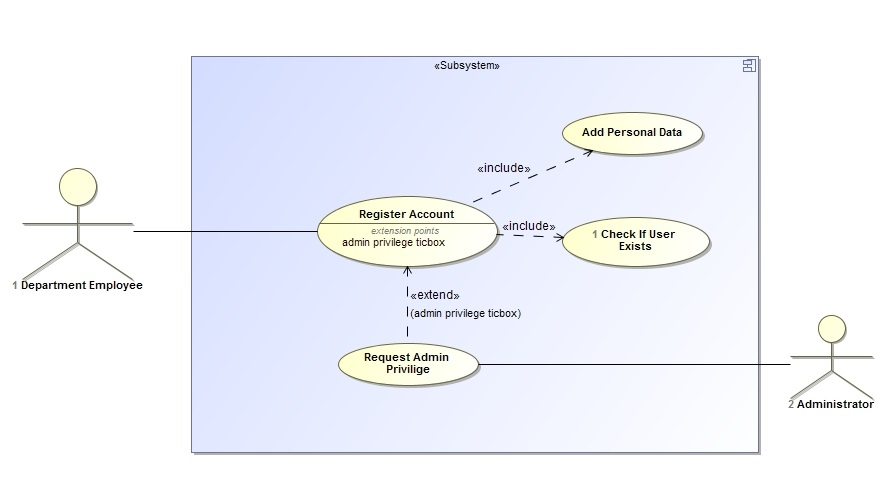
\includegraphics[width=1\textwidth]{./Registration.jpg}\\[1.5cm]
	 
	\subsubsection{Login Use Case Diagram}
	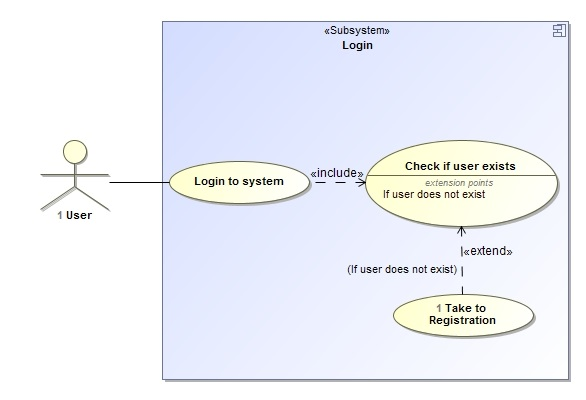
\includegraphics[width=1\textwidth]{./Login.jpg}\\[1.5cm] 
	
	\subsubsection{Logout Use Case Diagram}
	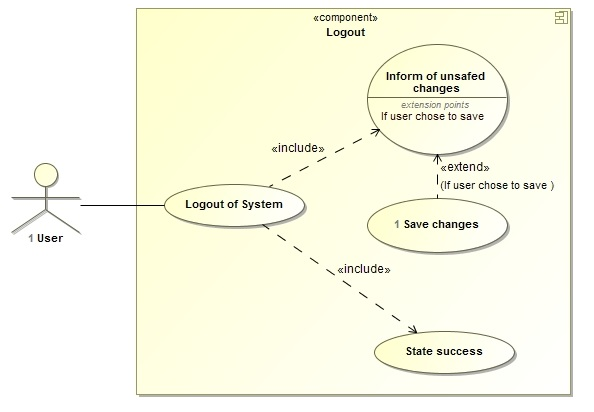
\includegraphics[width=1\textwidth]{./Logout.jpg}\\[1.5cm]
	
	\subsubsection{Create Publication Use Case Diagram}
	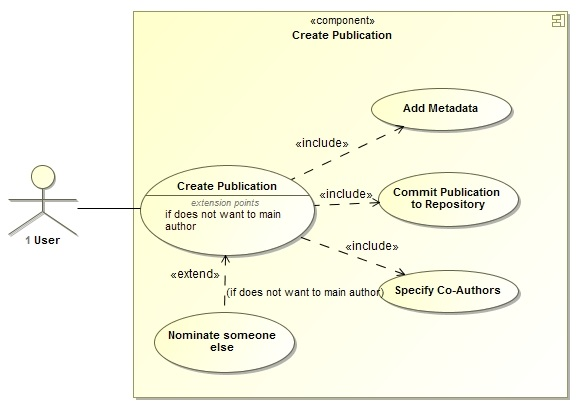
\includegraphics[width=1\textwidth]{./CreatePublication.jpg}\\[1.5cm]

	\subsubsection{Add/Remove Author Use Case Diagram}
	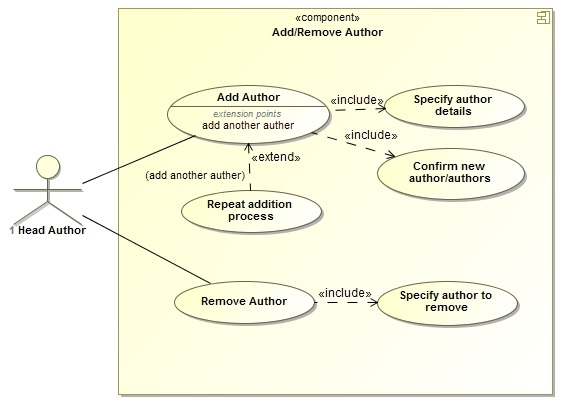
\includegraphics[width=1\textwidth]{./AddRemoveAuthor.jpg}\\[1.5cm]

	\subsubsection{Edit Publication Use Case Diagram}
	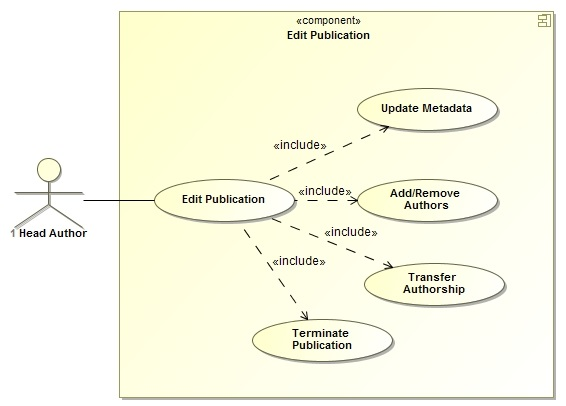
\includegraphics[width=1\textwidth]{./EditPublication.jpg}\\[1.5cm]

	\subsubsection{View Publication Use Case Diagram}
	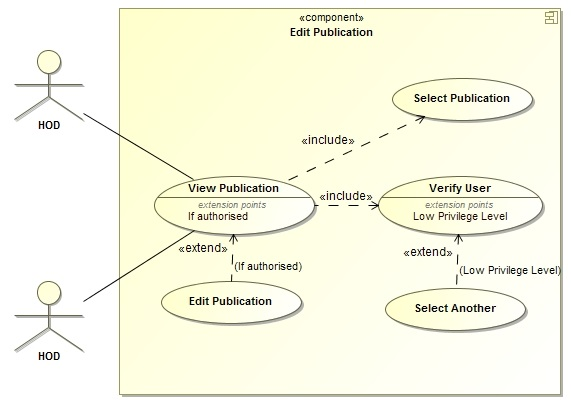
\includegraphics[width=1\textwidth]{./ViewPublication.jpg}\\[1.5cm]
		
\subsection{Process specifications}
\subsection{Domain Model}

\newpage
\section{References}

\end{document}
